\documentclass[12pt,a4paper]{article}
\usepackage{bold-extra}
\usepackage{appendix}
\usepackage{amsfonts,amsmath,amssymb}
\usepackage{enumerate}
\usepackage{float}
\usepackage{geometry}
\usepackage{graphicx}
\usepackage{latexsym}
\usepackage{listings}
\usepackage{multicol,multirow}
\usepackage{subfigure}
\usepackage{tabularx}
\usepackage{ulem}
\usepackage{tikz}
\usepackage{xcolor}
\geometry{a4paper,left=1in,right=1in,top=1in,bottom=1in}
\begin{document}
\centerline{\Huge{{\textbf{PHYSICS I\ \ Problem Set 3}}}}
\vspace{0.5cm}
\leftline{\large{Name: Haotian Fu}}
\rightline{\large{Student ID: 520021910012}}
\paragraph{\large \textbf{Problem 1}}~{\textbf{Solution}}
\vspace{2mm}\\
\noindent (a) Since the tangential component of the particle's acceleration is a constant, we may as well suppose this constant as $a_\tau$. Then $v_{(t)} = a_\tau t$.
\par For polar coordinate system, $\bar{a} = (\mathop{r}\limits^{\cdot\cdot}-r(\mathop{\varphi}\limits^\cdot)^2)\hat{n}_r + (r\mathop{\varphi}\limits^{\cdot\cdot}+2\mathop{r}\limits^{\cdot}\mathop{\varphi}\limits^{\cdot})\hat{n}_\varphi$
\par In circular motion we know
\begin{align*}
	r = \text{R} = \text{constant}\quad &\text{Hence} \mathop{r}\limits^{\cdot} = \mathop{r}\limits^{\cdot\cdot} =0 \\
	\text{Besides, radial} &= \text{normal} 
\end{align*}
\par Therefore, $\lvert\bar{a}_n\rvert$ = $r(\mathop{\varphi}\limits^\cdot)^2$. Note that $\bar{v} = \mathop{r}\limits^\cdot\hat{n}_r + r\mathop{\varphi}\limits^\cdot\hat{n}_\varphi$, namely, $v = r\mathop{\varphi}\limits^\cdot$. We rewrite 
\begin{align*}
	\lvert\bar{a}_n\rvert_{(t)} = \frac{v^2}{R} = \frac{a_\tau^2 t^2}{R}
\end{align*}
\noindent (b) According to (a), we have $\lvert\bar{a}_n\rvert_{(t)} =\frac{a_\tau^2 t^2}{R}$. We then know
\begin{align*}
	\lvert\bar{a}_{(t)}\rvert = \sqrt{a_\tau^2 + a_n^2} = \sqrt{a_\tau^2 + (\frac{a_\tau^2 t^2}{R})^2} = \frac{a_\tau}{R} \sqrt{R^2 + a_\tau^2 t^4}
\end{align*}
\par Based on what we have calculated so far, we can easily calculate the angle $\theta$ that the vector \textbf{a} forms with the position vector \textbf{r}. Since \textbf{a} = $\bar{a}_n + \bar{a}_\tau$ and $\bar{r}$ is negative direction to $\bar{a}_n$, we have
\begin{align*}
	\cos\theta = \frac{\textbf{a}\cdot\textbf{r}}{\lvert\textbf{a}\rvert\cdot\lvert\textbf{r}\rvert} &= \frac{\bar{a_\tau}\bar{r} + \bar{a_n}\bar{r}}{\sqrt{a_\tau^2 + a_n^2} \cdot R} = \frac{-\lvert\bar{a}_n\rvert_{(t)}}{\sqrt{a_\tau^2 + a_n^2}} = \frac{-a_\tau t^2}{\sqrt{R^2 + a_{\tau}^2 t^4}}\\
	\Rightarrow \quad
	\theta &= \arccos(\frac{-a_\tau t^2}{\sqrt{R^2 + a_{\tau}^2 t^4}})
\end{align*}

\paragraph{\large \textbf{Problem 2}}~{\textbf{Solution}}
\vspace{2mm}\\
\noindent (a) Set the ground as our frame of reference.
\par According to Newton's second law, since the magnitude and direction of the ball's velocity remains constant, the net force the ball exerted is zero. Therefore, angle that the string forms with the vertical direction is 0$^\circ$.\\ \\
\noindent (b) Suppose the magnitude of acceleration is \textit{a}. According to free body diagram(b), we have
\begin{align*}
	\left\{ \begin{array}{c}
		T\cos\theta = mg\\
		T\sin\theta = ma	
	\end{array} \right.
	\quad \Rightarrow \quad
	\theta = \arctan(\frac{a}{g})
\end{align*}
\par Therefore, the angle that the string forms with the vertical direction is $\arctan(\frac{a}{g})^\circ$.\\ \\
\noindent (c) Since the ball is attached to the roof of the car, it shares the same acceleration of that car. Then according to free body diagram(c), for the system we have
\begin{align*}
	\left\{ \begin{array}{c}
		T\cos(\theta - \alpha) = mg\cos\alpha\\
		m_{\text{ball}}a = m_{\text{ball}}g\sin\alpha + T\sin(\theta - \alpha)\\
		m_{\text{car}}a = m_{\text{car}}g\sin\alpha\\			
	\end{array} \right.	
	\quad \Rightarrow \quad
	\left\{ \begin{array}{c}
		\theta = \alpha\\
		T = mg
	\end{array} \right.
\end{align*}
\begin{figure}[H]
    \centering
    \subfigure[Constant speed along a straight line]{
    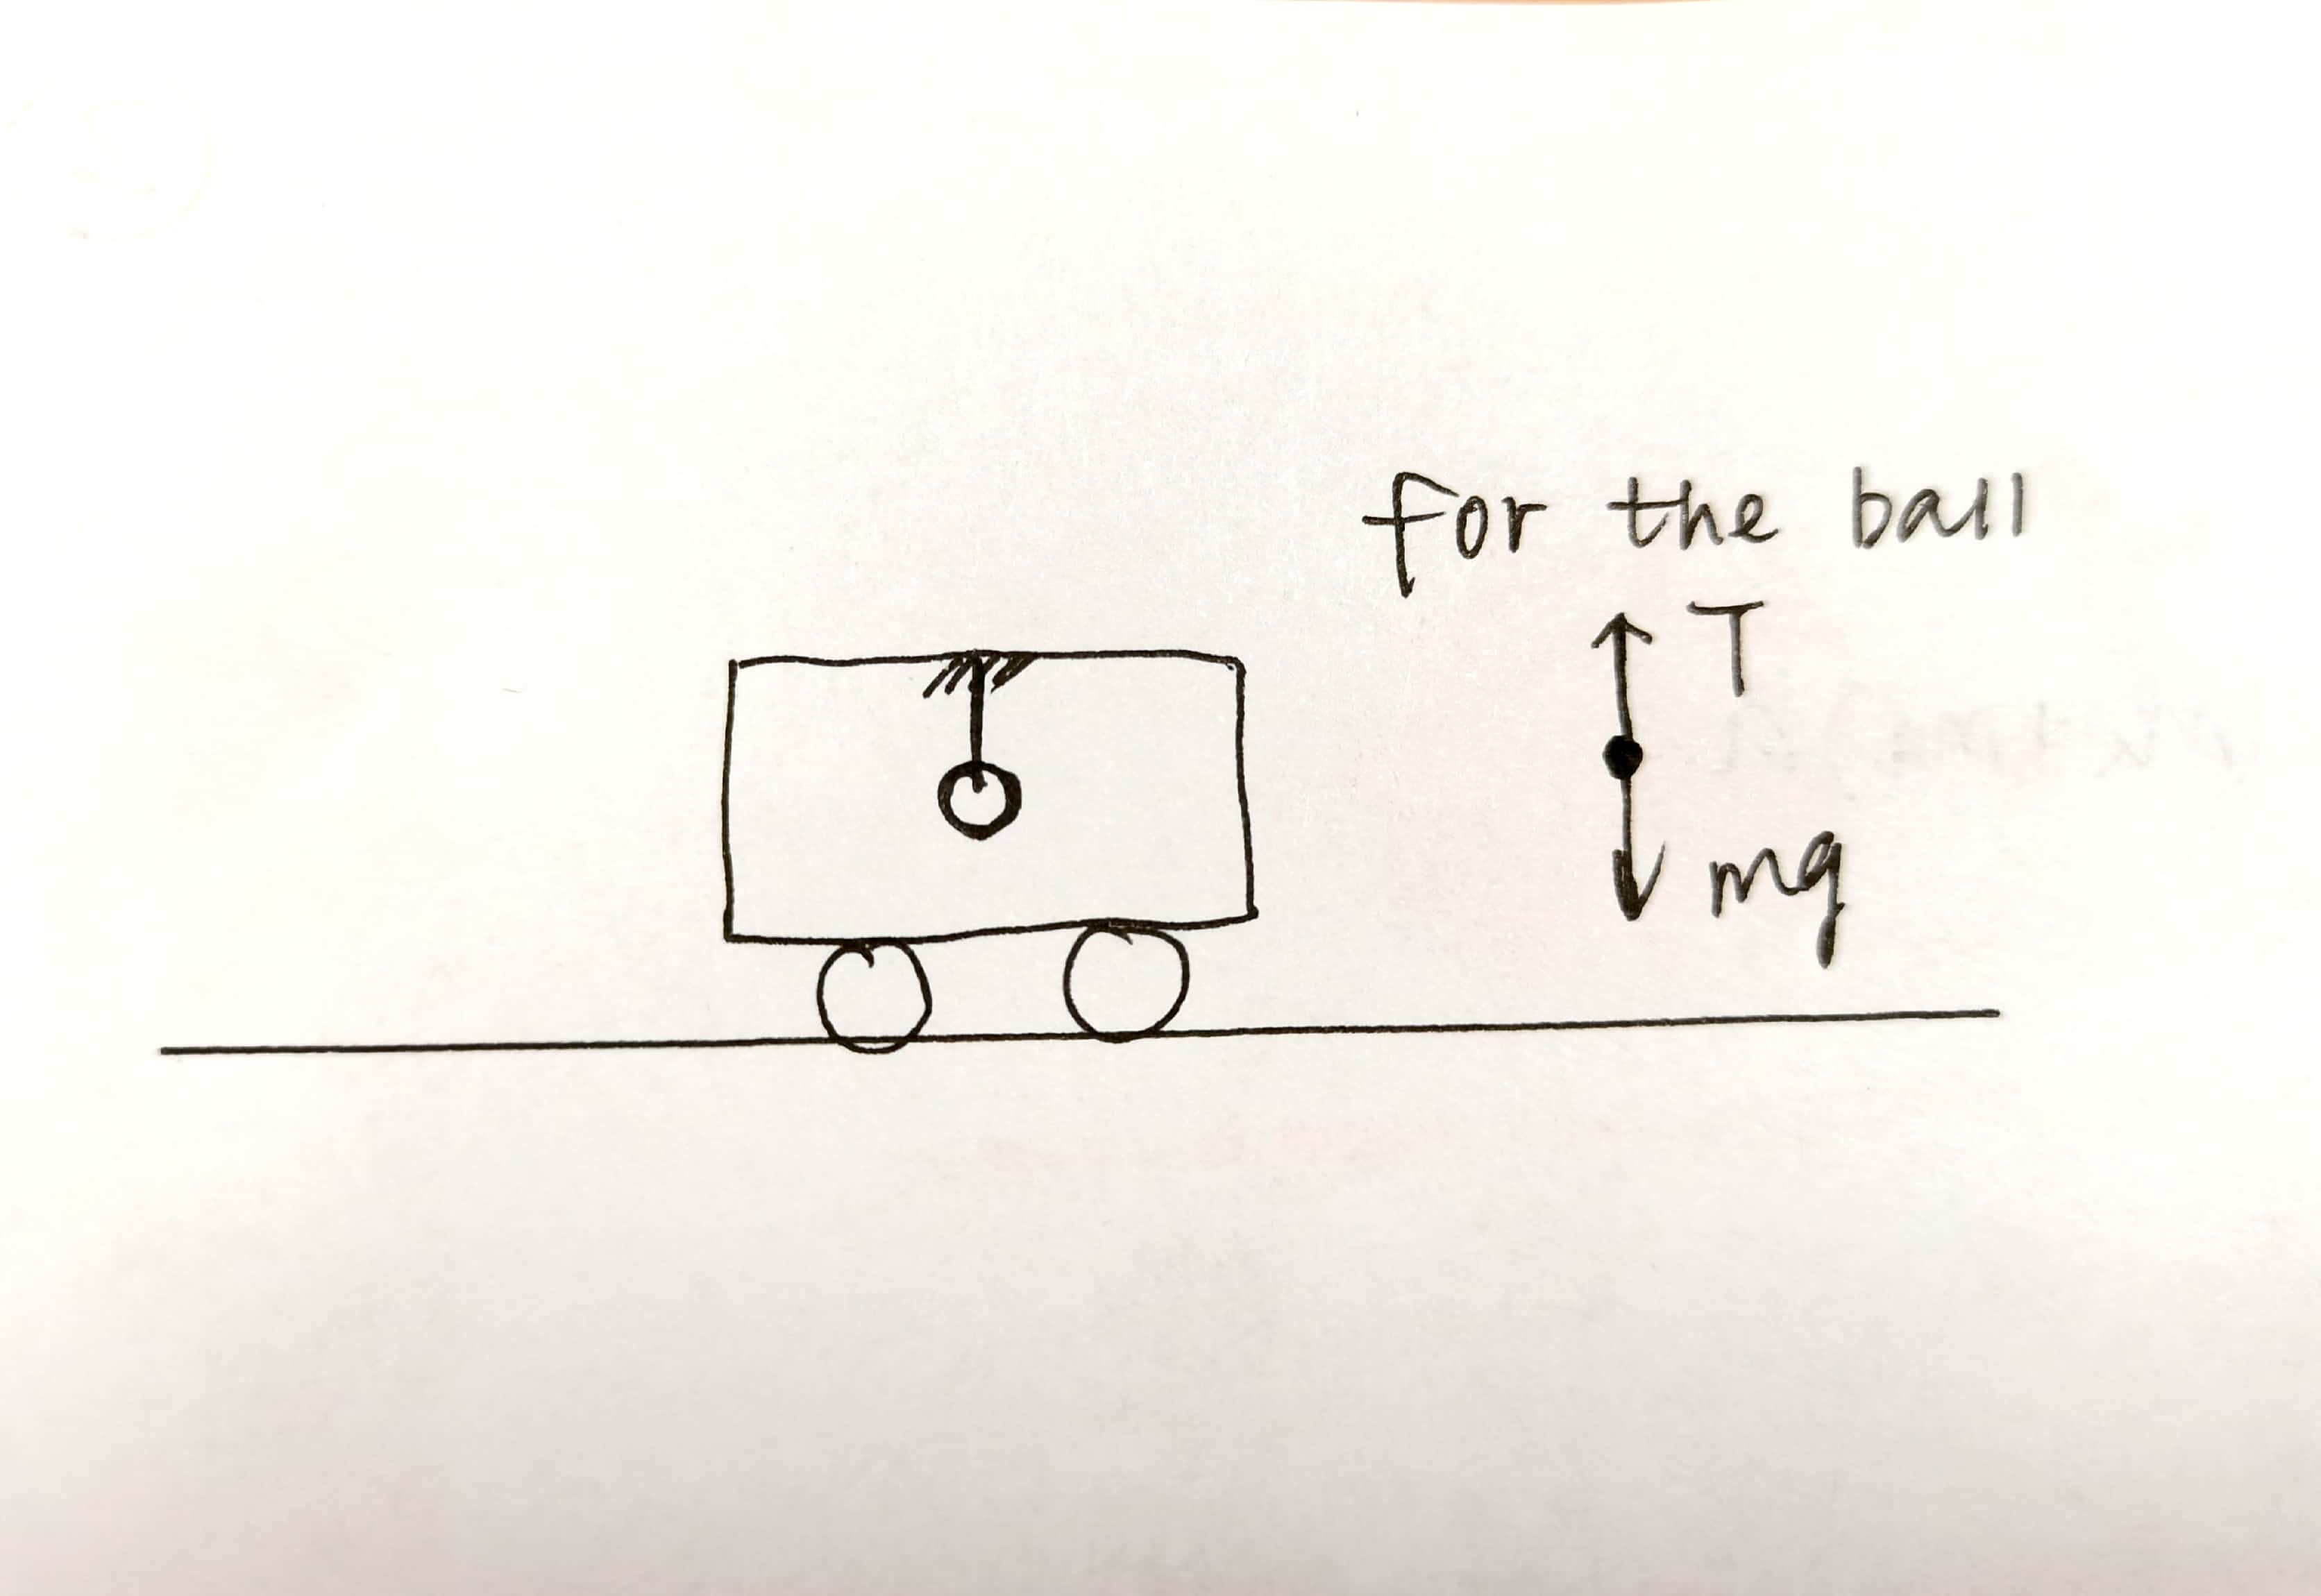
\includegraphics[height = 3cm]{1.jpg}
    }
    \subfigure[Constant acceleration along a straight line]{
    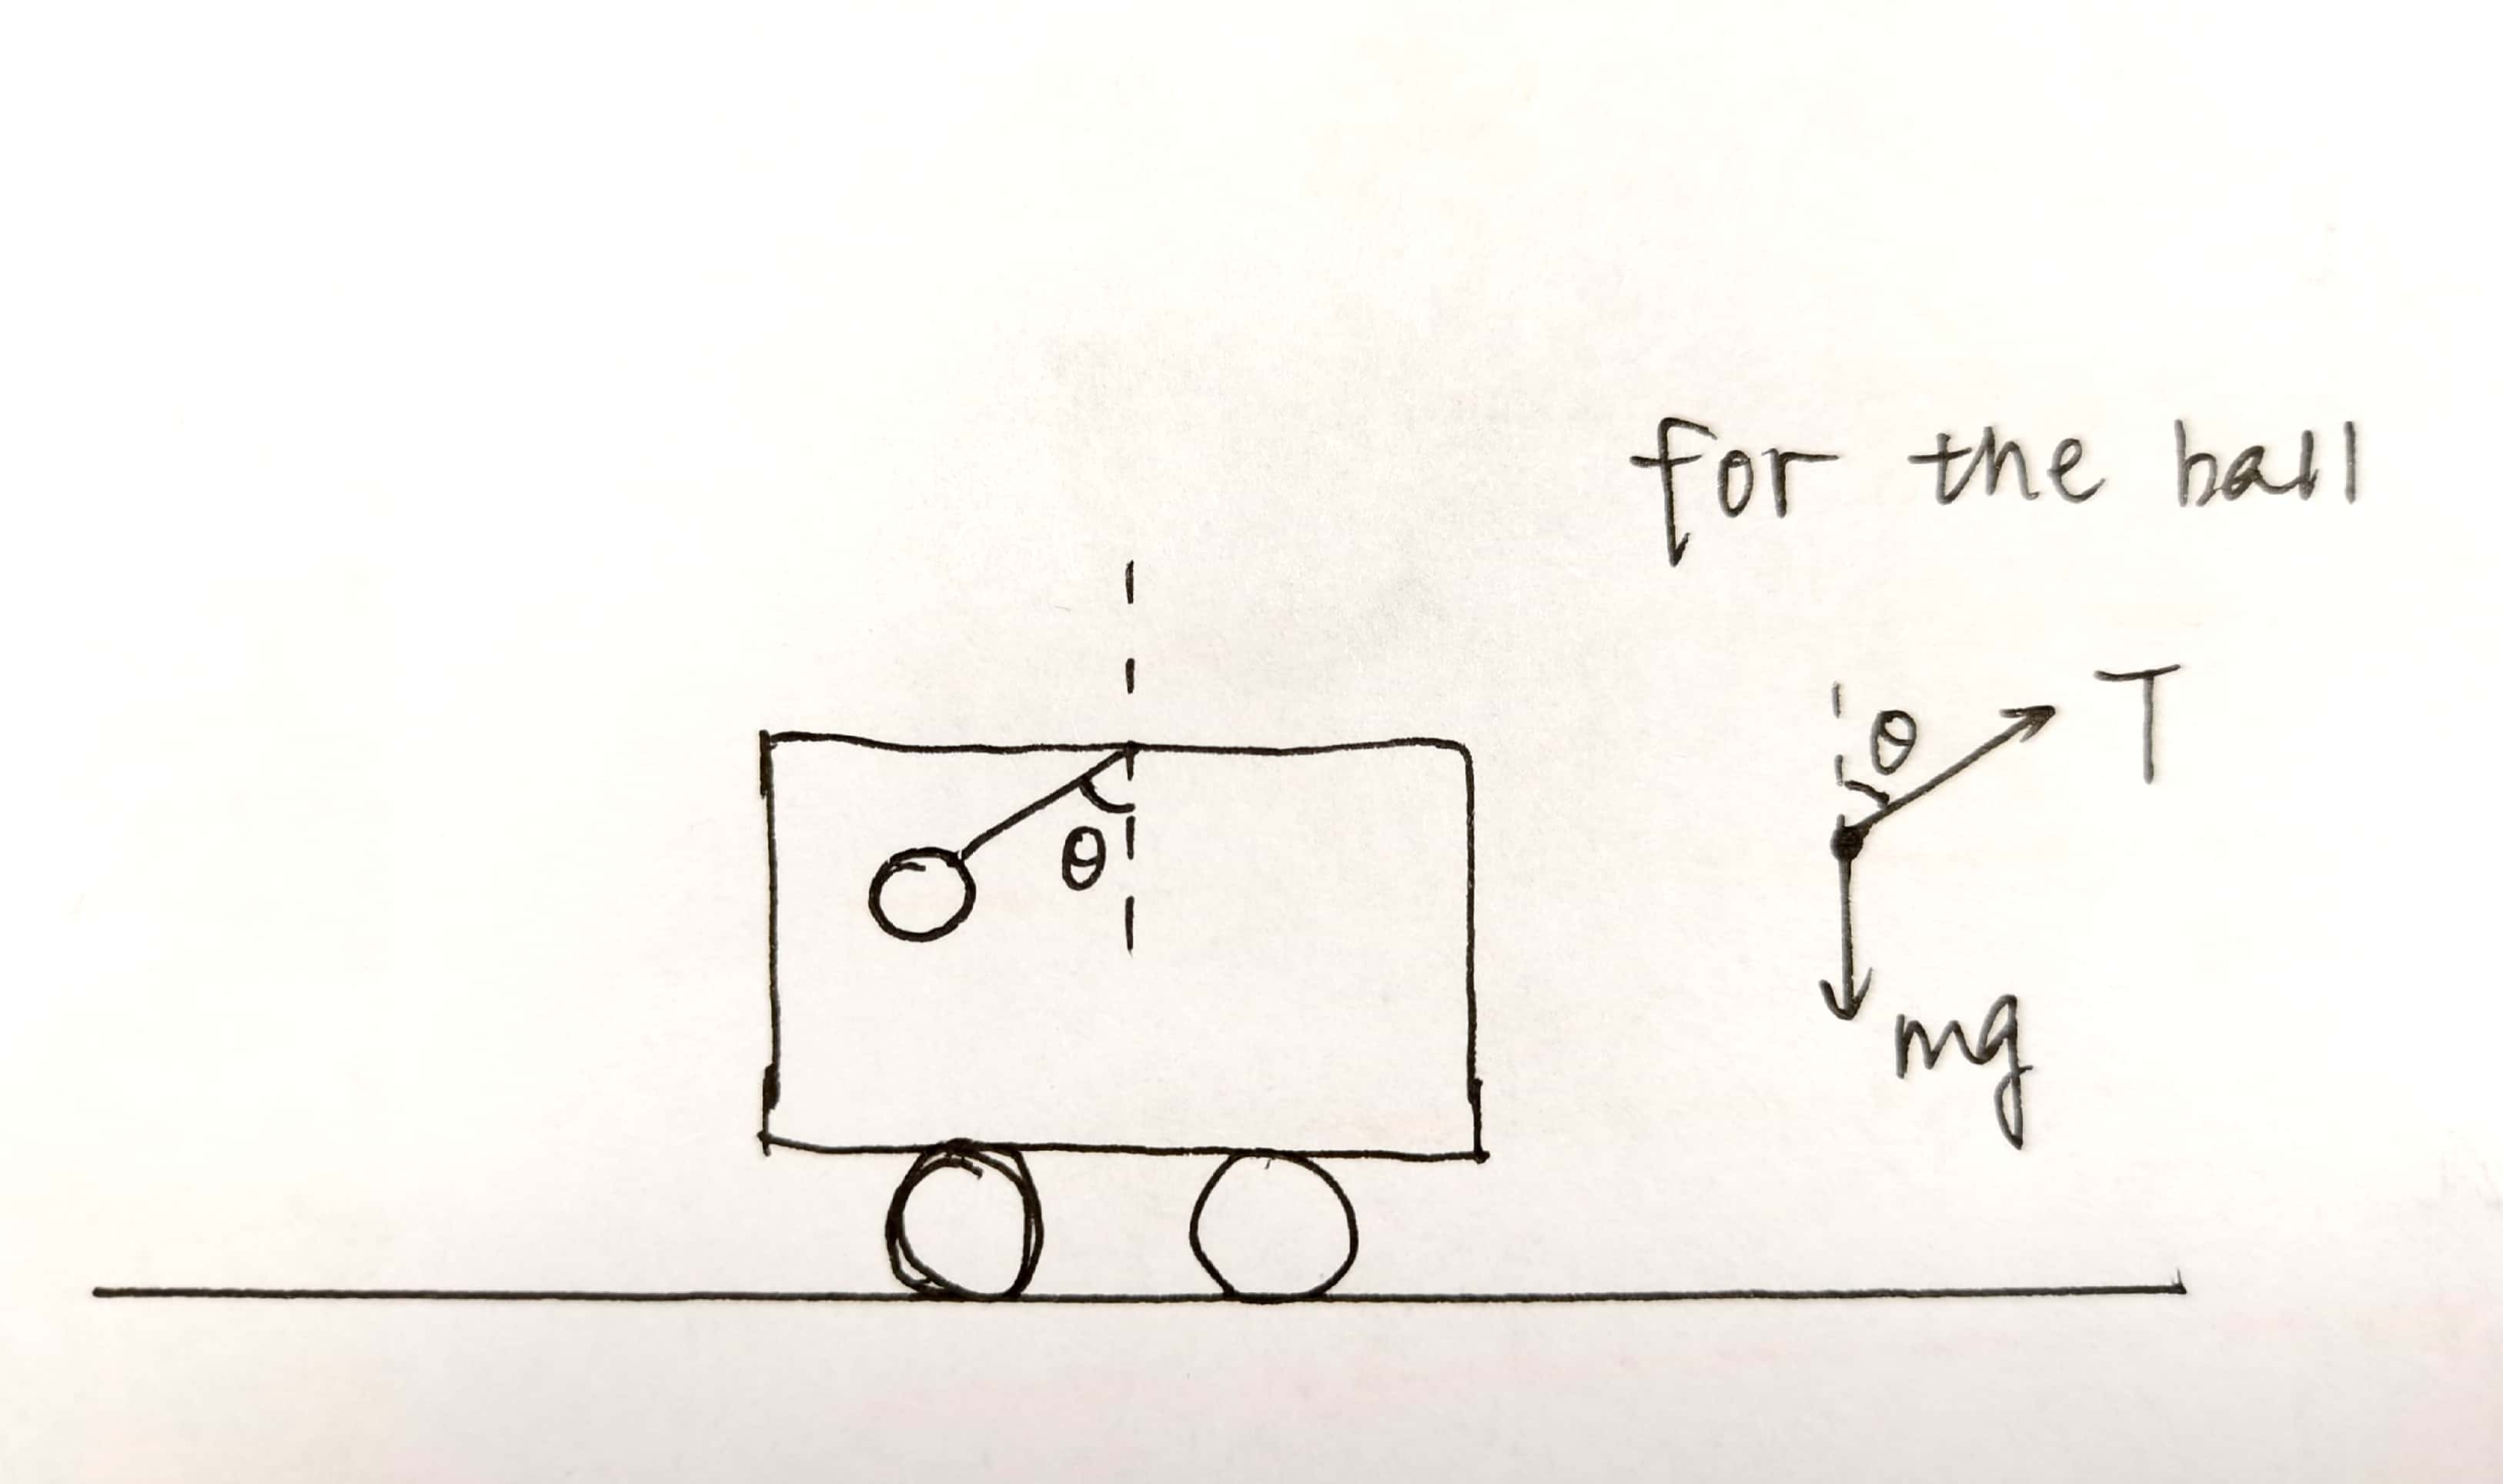
\includegraphics[height = 3cm]{2.jpg}
    }
    \subfigure[Sliding down a slide]{
    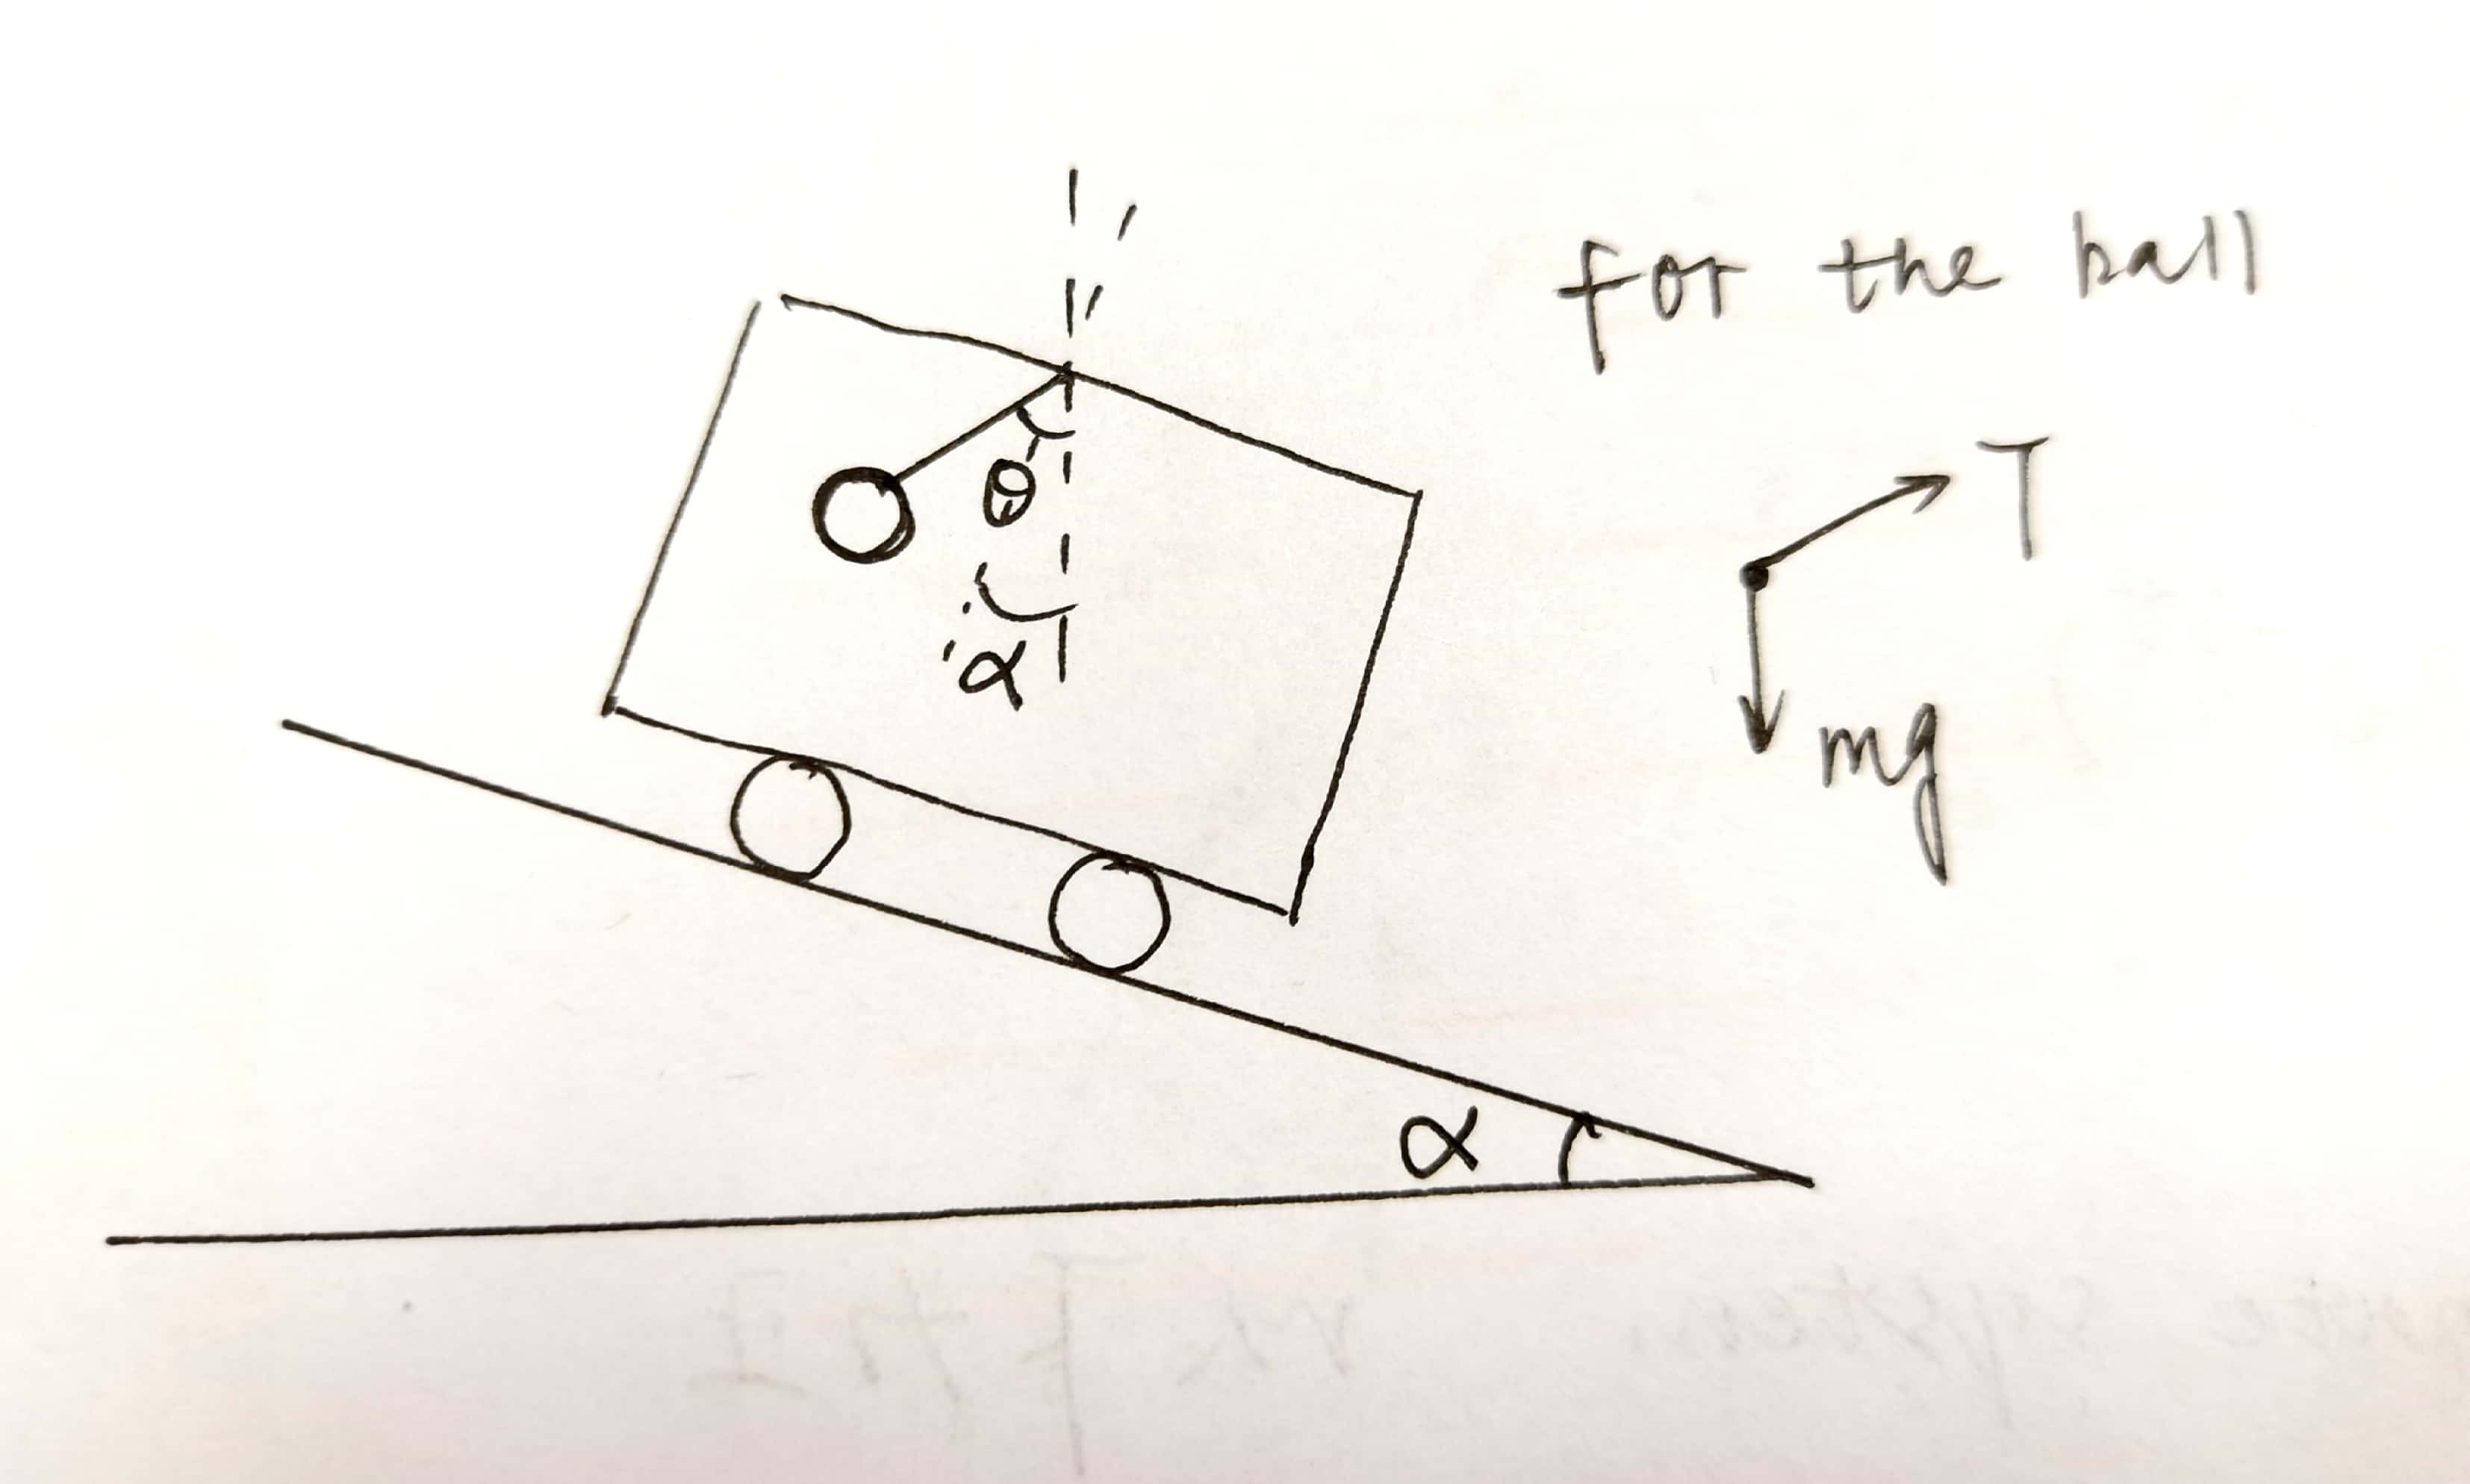
\includegraphics[height = 3cm]{3.jpg}
    }
    \caption{Free body diagrams in Problem 2}
\end{figure}

\paragraph{\large \textbf{Problem 3}}~{\textbf{Solution}}
\vspace{2mm}\\
\noindent (a) We first consider $m_1$ and $m_2$ as a whole, and then draw the free body diagram of $m_3$ and the system of $m_1$ and $m_2$. Then we have
\begin{align*}
	m_3 a &= m_3g\sin2\alpha - T_3\\
	(m_1 + m_2)a = T_3 - (m_1 &+ m_2)g\sin\alpha - \mu_1m_1g\cos\alpha - \mu_2m_2g\cos\alpha
\end{align*}
$\Rightarrow$
\begin{align*}
	a &= \frac{m_3g\sin2\alpha - (m_1 + m_2)g\sin\alpha - \mu_1m_1g\cos\alpha - \mu_2m_2\cos\alpha}{m_1 + m_2 + m_3}\\
	T_3 &= \frac{m_3}{m_1 + m_2 + m_3}\cdot \left(
		(m_1 + m_2)(\sin2\alpha + \sin\alpha)g + \mu_1m_1g\cos\alpha + \mu_2m_2g\cos\alpha
	\right)
\end{align*}
\par Then we analyze $m_1$ and $m_2$ separately
\begin{align*}
	m_2a &= T_2 - T_1 - m_2g\sin\alpha - \mu_2m_2g\cos\alpha\\
	m_1a &= T_1 - m_1g\sin\alpha - \mu_1m_1g\cos\alpha
\end{align*}
$\Rightarrow$
\begin{align*}
	T_1 &= \frac{m_1}{m_1 + m_2 + m_3}\cdot \left(
		m_3g\sin2\alpha + m_3g\sin\alpha + \mu_1m_3g\cos\alpha + \mu_1m_2g\cos\alpha - \mu_2m_2g\cos\alpha
	\right)\\
	T_2 &= \frac{m_3g}{m_1 + m_2 + m_3}\cdot \left(
		(m_1 + m_2)(\sin2\alpha + \sin\alpha) + (\mu_1m_1 + \mu_2m_2)\cos\alpha
	\right)
\end{align*}
\noindent (b) Since acceleration and tensions cannot be negative and denominator cannot be zero, we have
\begin{align*}
	m_3\sin2\alpha\ \textgreater\ (m_1 + m_2)\sin\alpha &+ \mu_1m_1\cos\alpha + \mu_2m_2\cos\alpha\\
	m_3 - m_1 &- m_2\ \textgreater\ 0\\
	\mu_1m_1g\cos\alpha\ &\leq\ m_1g\sin\alpha\\
	\mu_2m_2g\cos\alpha\ &\leq\ m_2g\sin\alpha
\end{align*}
$\Rightarrow$
\begin{align*}
	m_3\ \textgreater\ \frac{m_1 + m_2}{2\cos\alpha} + \frac{\mu_1m_1 + \mu_2m_2}{2\sin\alpha}\quad \text{and} \quad \mu_1\ \leq\ \tan\alpha\quad \text{and} \quad \mu_2\ \leq\ \tan\alpha
\end{align*}
\begin{figure}[H]
    \centering
    \subfigure[Free body diagram of $m_3$ and the system of $m_1$ and $m_2$]{
    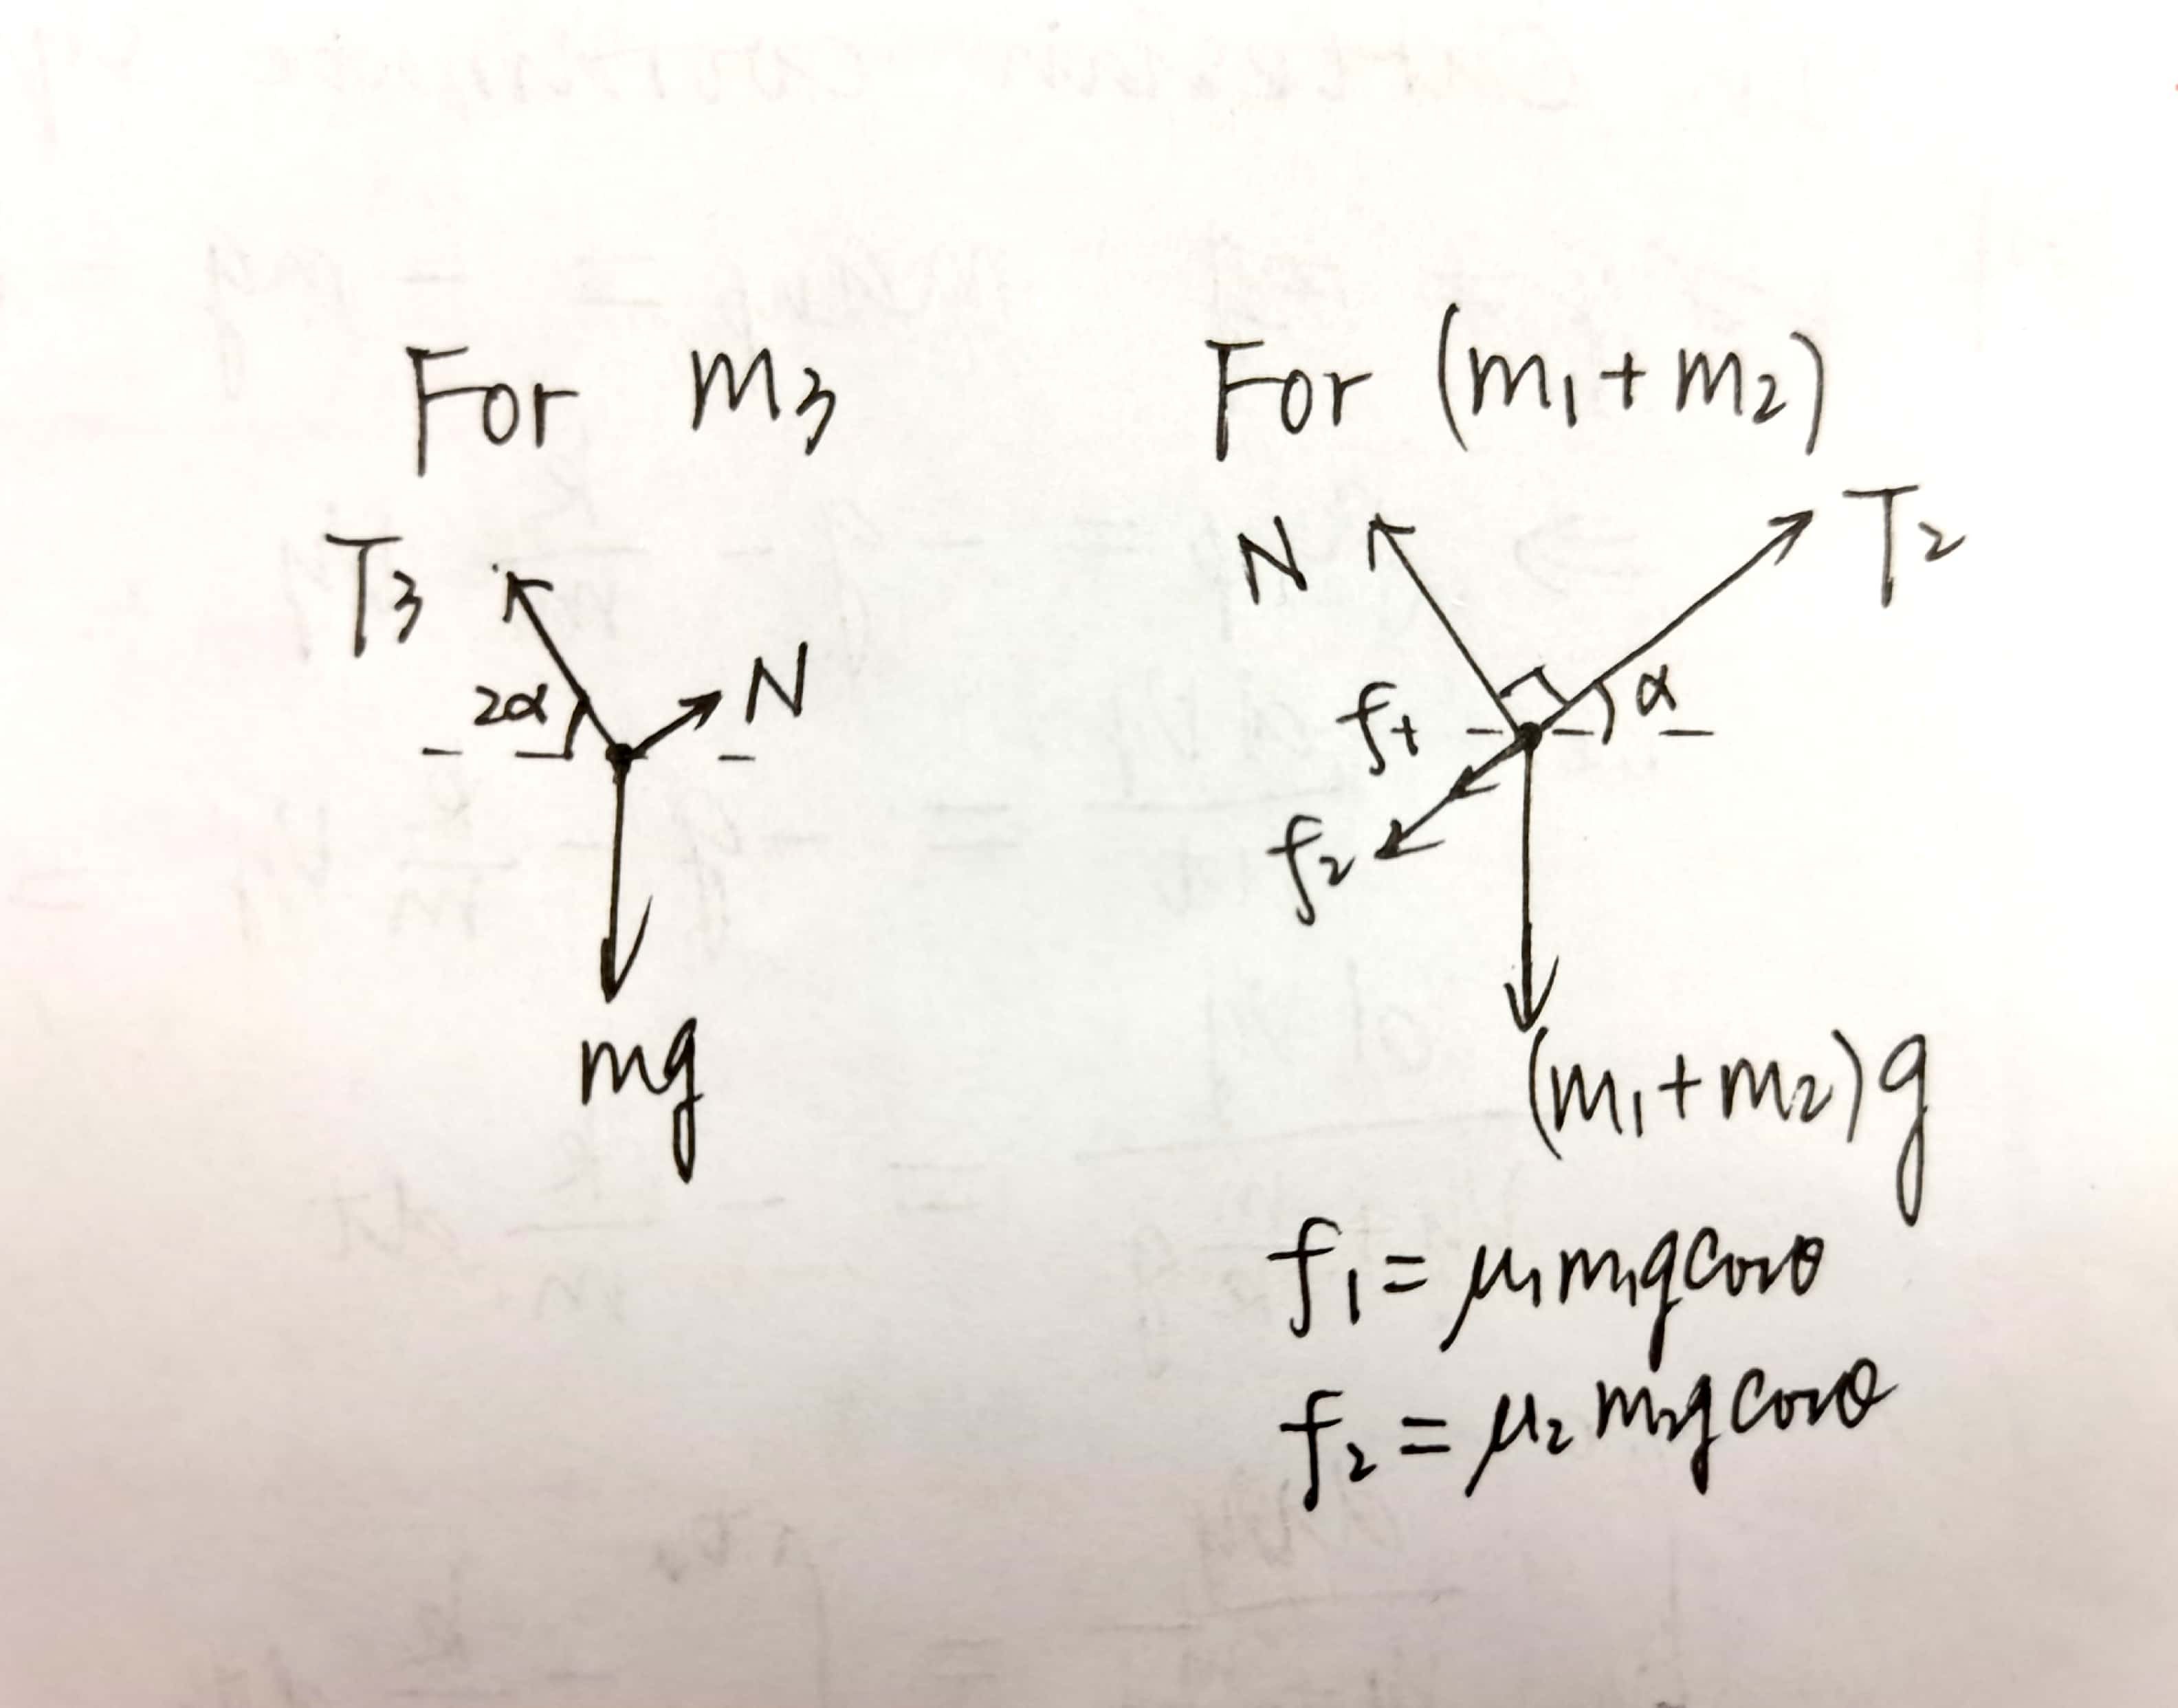
\includegraphics[height = 5cm]{4.jpg}
    }
    \subfigure[Free body diagram of $m_1$ and $m_2$]{
    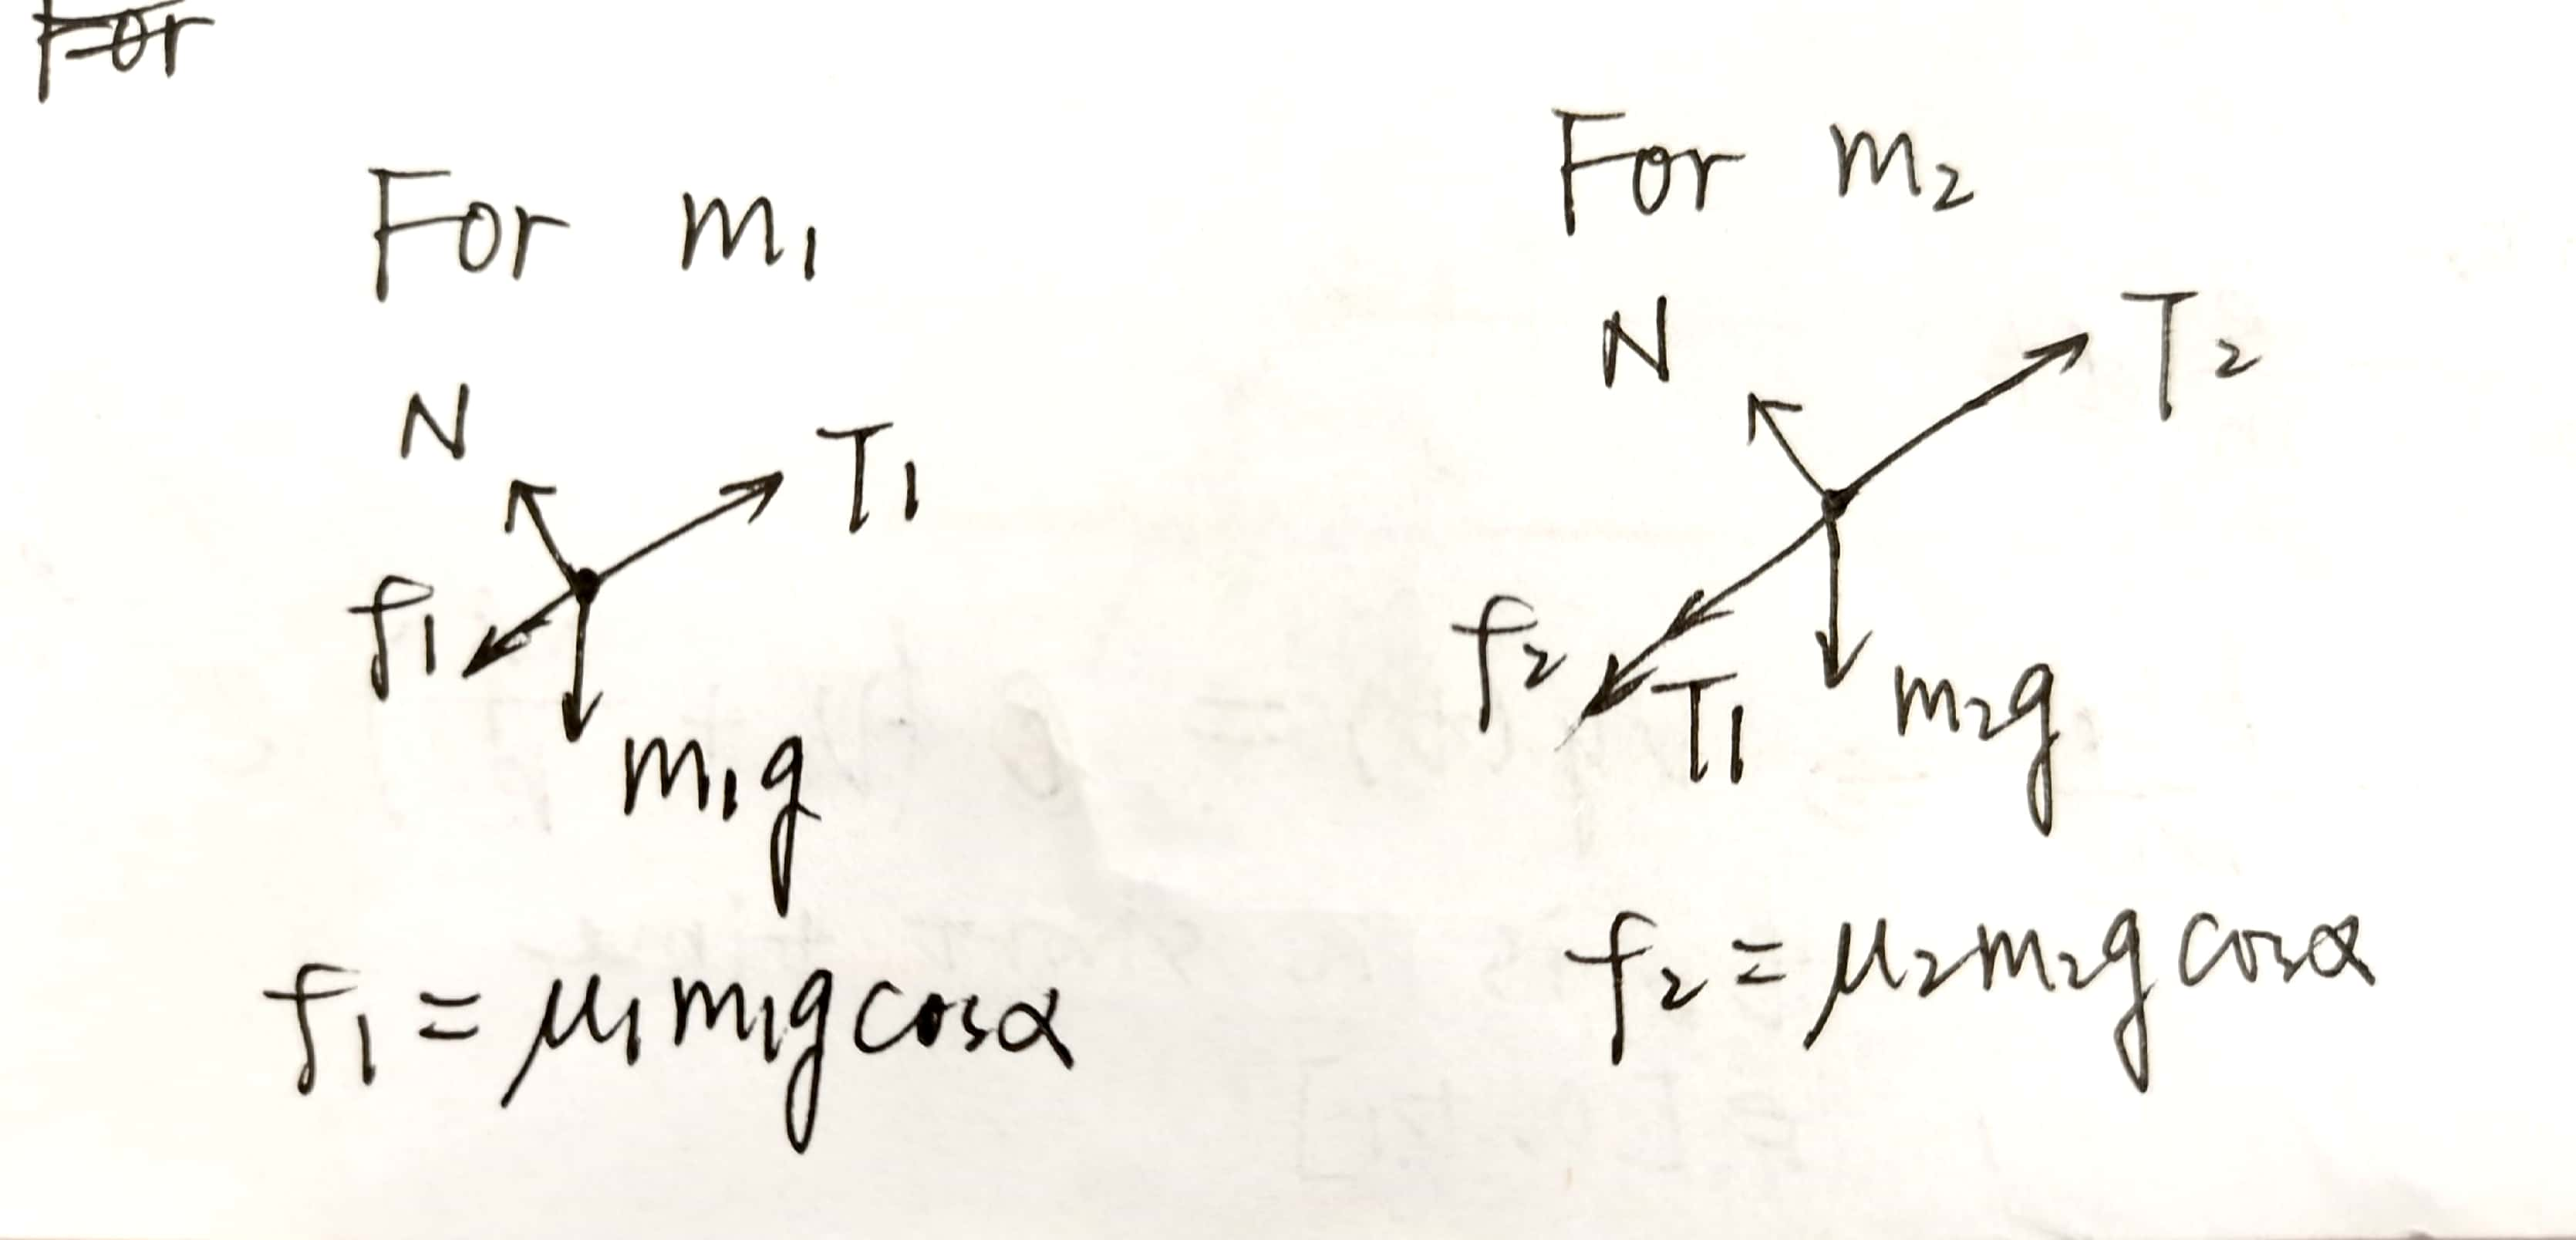
\includegraphics[height = 3cm]{5.jpg}
    }
    \caption{Free body diagrams in Problem 3}
\end{figure}

\paragraph{\large \textbf{Problem 4}}~{\textbf{Solution}}
\vspace{2mm}
\par Set the upwards as the positive direction.\\
\noindent (a) According to Newton's third law, the rope gives the student a reactive force when the student exerts an acting force on the rope, namely, $F' = F$. We draw a free body diagram and analyze the student and the bar as a whole system.
\par According to the diagram, suppose the rope around pulley exerts \textit{T} on the bar, the mass of the student is $m_1$, the mass of the bar is $m_2$, we have
\begin{align*}
	\left\{ \begin{array}{c}
		T = F'\\
		(m_1 + m_2) a = T + F' - (m_1 + m_2)g
	\end{array} \right.	
	\quad \Rightarrow \quad
	a = \frac{5}{12}\ m/s^2 = 0.417\ m/s^2
\end{align*}
\noindent (b) We then analyze the bar only
\par Suppose the force the student exerts on the bar is $F_T$. According to the free body diagram, we have
\begin{align*}
	m_2a = F_T - m_2g + T\\
\Rightarrow
	F_T = \frac{250}{3} N = -83.3 N
\end{align*}
\par Namely, the magnitude of $F_T$ is 83.3 \textit{N}, with pointing downwards.
\begin{figure}[H]
    \centering
    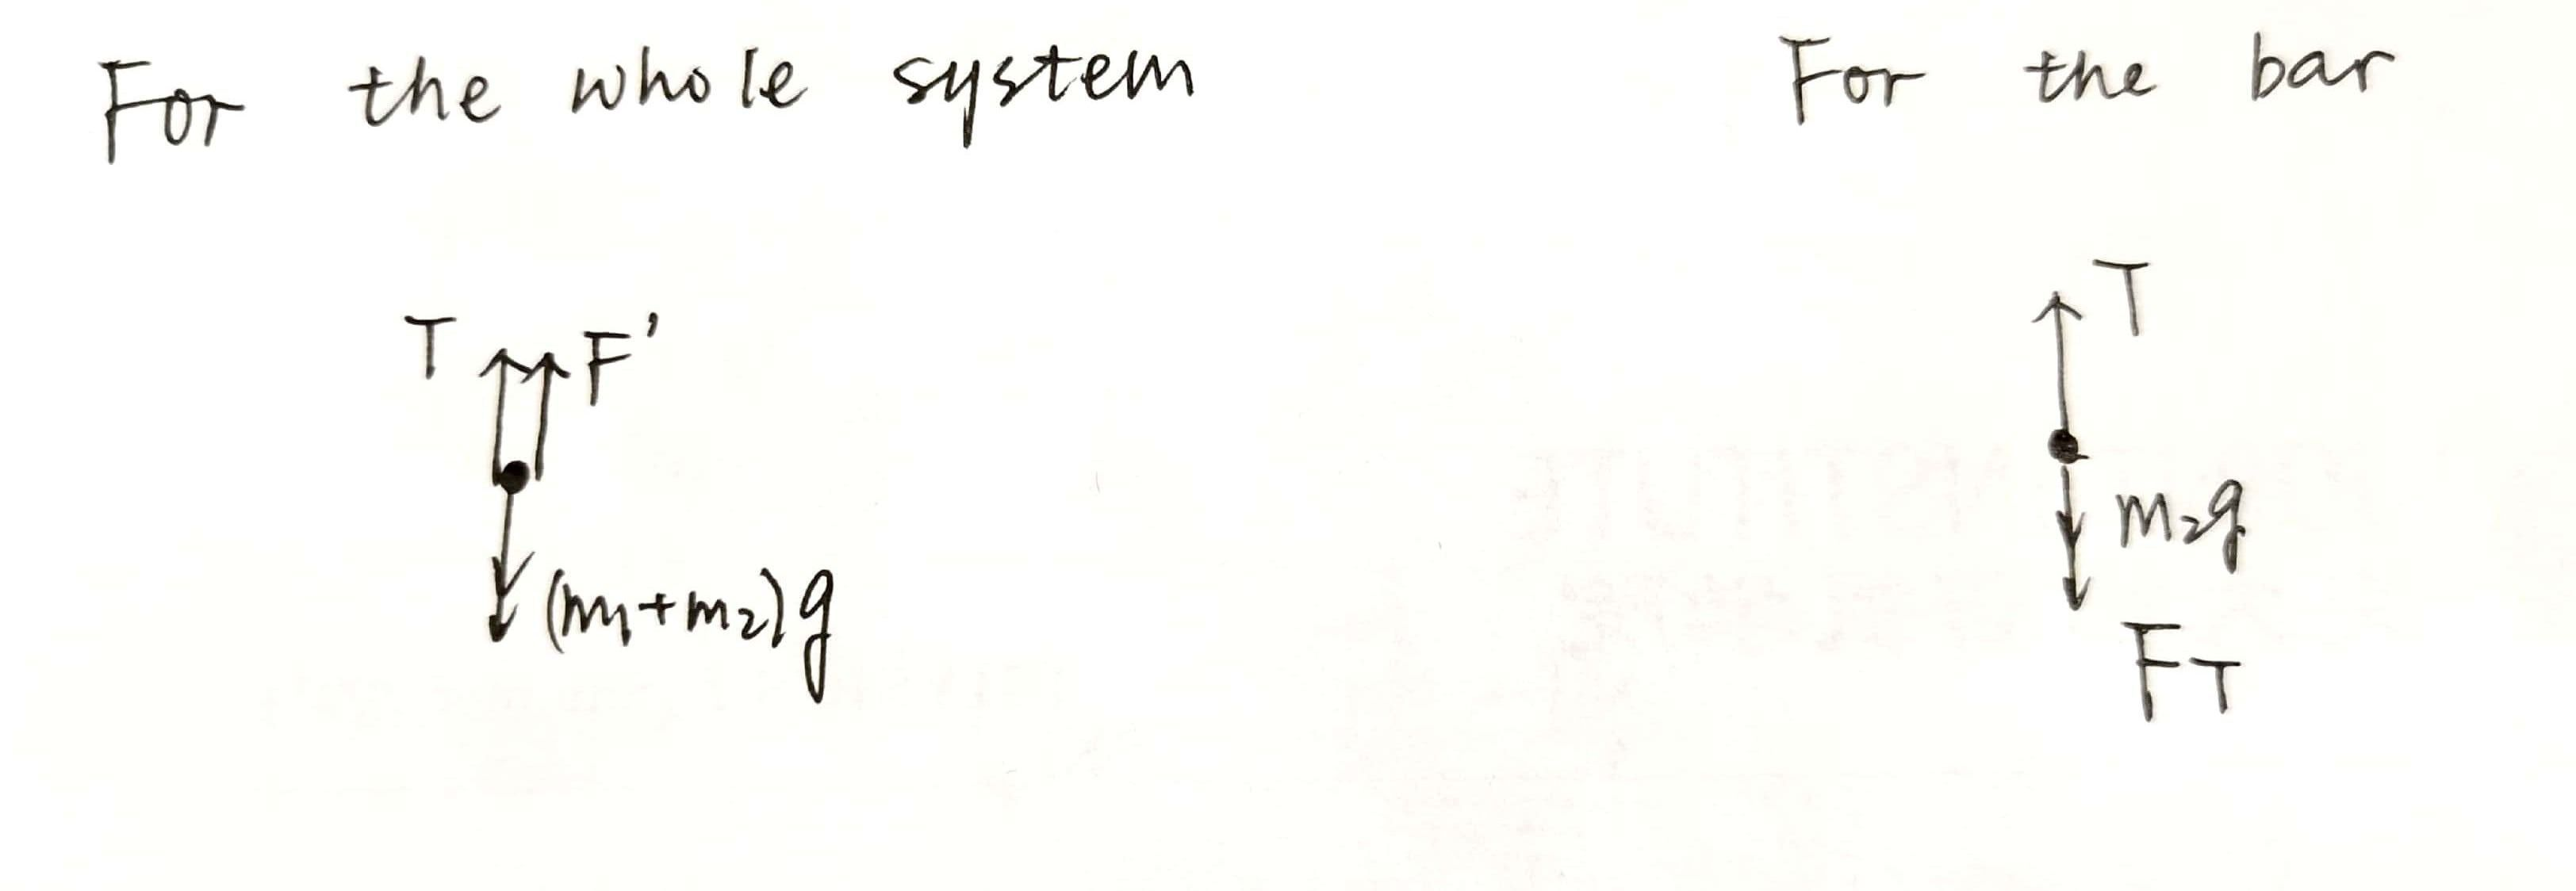
\includegraphics[height = 4cm]{6.jpg}
    \caption{Free body diagrams in Problem 4}
\end{figure}

\paragraph{\large \textbf{Problem 5}}~{\textbf{Solution}}
\vspace{2mm}
\par For the whole system
\begin{align*}
	F - \mu_kMg = (m+M) a\quad\Rightarrow\quad a = \frac{F - \mu_kMg}{m+M}
\end{align*}
\par Denote the tension as \textit{T} and the distance from the block is \textit{x}. For the rope
\begin{align*}
	T - \mu_kMg &= (\frac{m}{d}\cdot x + M) a\\
	\Rightarrow \quad T = \frac{mF - \mu_kmMg}{md + Md} &\cdot x + \frac{\mu_kmMg + MF}{m + M}
\end{align*}

\paragraph{\large \textbf{Problem 6}}~{\textbf{Solution}}
\vspace{2mm}
\par According Newton's second law
\begin{align*}
	ma &= F\\
\Rightarrow\quad \bar{a} = (2\sin&2t, 3t-6, -3e^{-3t})
\end{align*}
\par The integrate!
\begin{align*}
\left\{ \begin{array}{c}
		\int_{v(0)}^{v(t)}dv = \int_0^t\bar{a} dt\\
		\int_{r(0)}^{r(t)}dr = \int_0^t\bar{v} dt\\
	\end{array} \right.	
	\quad \Rightarrow \quad	
	\begin{array}{c}
		v(t) = (3-\cos2t, \frac{3}{2}t^2-6t, e^{-3t})\\
		r(t) = (-\frac{1}{2}\sin2t+3t+5, \frac{1}{2}t^3-3t^2+2, -\frac{1}{3}e^{-3t}-\frac{8}{3})
	\end{array}		
\end{align*}

\paragraph{\large \textbf{Problem 7}}~{\textbf{Solution}}
\vspace{2mm}
\par We set upwards as the positive direction.
\par \textbf{\textcolor{blue}{1)}} We first calculate the uprising procedure of the ball. According to Newton's second law
\begin{align*}
	ma_u &= - mg - kv_y\\
\Rightarrow \quad \quad a_u &= -(g + \frac{k}{m}v_y)
\end{align*}
\par Notice that $a_u = \frac{dv_y}{dt}$, we then get
\begin{align*}
	a_u = \frac{dv_y}{dt} = -g - \frac{k}{m}v_y &= -\frac{k}{m}\left( v_y + \frac{m}{k}g \right)\\
	\frac{dv_y}{v_y + \frac{m}{k}g} &= -\frac{k}{m}dt\\
	\int_{v_0}^{v_{y(t)}} \frac{dv_y}{v_y + \frac{m}{k}g} &= \int_0^{t} \frac{k}{m}dt\\
	ln \left( \frac{v_{y(t)} + \frac{m}{k}g}{v_0 + \frac{m}{k}g} \right) &= \frac{-kt}{m}\\
\Rightarrow\quad \quad v_{y_{(t)}} &= \left( v_0 + \frac{mg}{k} \right) e^{\frac{-kt}{m}} - \frac{mg}{k}
\end{align*}
\par Analougously, we can calculate the $y_{(t)}$ as follows
\begin{align*}
	v_{y(t)} = \frac{dy_{(t)}}{dt} = \left( v_0 + \frac{mg}{k} \right) e^{-\frac{kt}{m}} - \frac{mg}{k}\\
	\int_0^{y_{(t)}} dy = \int_0^t \left( \left( v_0 + \frac{mg}{k} \right) e^{-\frac{kt}{m}} - \frac{mg}{k} \right) dt\\
	y_{(t)} = \left( v_0 + \frac{mg}{k} \right) \int_0^t e^{-\frac{kt}{m}} - \int_0^t \frac{mg}{k} dt\\
	y_{(t)} = -\left( \frac{mv_0}{k} + \frac{m^2g}{k^2} \right) e^{-\frac{kt}{m}} - \frac{mg}{k}t + \frac{m^2g}{k^2} + \frac{mv_0}{k}
\end{align*}
\vspace{4mm}
\par Suppose the time when the ball reaches its highest point is $t_s$, then $v_{y(t_s)} = 0$. Namely
\begin{align*}
	\left( v_0 + \frac{mg}{k} \right) e^{-\frac{kt}{m}} - \frac{mg}{k} = 0\\
\Rightarrow\quad \quad t_s = \frac{m}{k}\ ln \left( \frac{mg/k + v_0}{mg/k} \right)
\end{align*}
\par Therefore, the highest point of the ball's trajectory is
\begin{align*}
	h_{max} &= \lvert y_{(t_s)}\rvert = -\left( \frac{m^2g}{k^2} + \frac{mv_0}{k} \right)\cdot \frac{mg/k}{mg/k + v_0} - \frac{m^2g}{k^2}ln \left( \frac{mg/k + v_0}{mg/k} \right) + \frac{m^2g}{k^2} + \frac{mv_0}{k}\\ &= \frac{mv_0}{k} - \frac{m^2g}{k^2}ln \left( \frac{mg/k + v_0}{mg/k} \right) 
\end{align*}
\vspace{4mm}
\par \textbf{\textcolor{blue}{2)}} We then calculate the falling procedure of the ball. Set downwards the positive disrection. According to Newton's second law
\begin{align*}
	ma_d &= mg - kv_y\\
\Rightarrow \quad \quad a_d &= g - \frac{k}{m}v_y
\end{align*}
\par Analogously, we get
\begin{align*}
	v_{y(t)} &= \frac{mg}{k} - \frac{mg}{k}e^{-\frac{k}{m}(t-\frac{m}{k}\ ln \left( \frac{mg/k + v_0}{mg/k} \right))} = \frac{mg}{k} - (\frac{mg}{k}+v_0)e^{-\frac{kt}{m}}\\
	y_{(t)} &= \frac{m^2g}{k^2}e^{-\frac{k}{m}(t-\frac{m}{k}\ ln \left( \frac{mg/k + v_0}{mg/k} \right))} + \frac{mg}{k}(t-\frac{m}{k}\ ln \left( \frac{mg/k + v_0}{mg/k} \right)) - \frac{m^2g}{k^2} + h_{max}\\
	&= \frac{m^2g}{k^2}\cdot \frac{mg+kv_0}{mg} e^{-\frac{kt}{m}} + \frac{mg}{k} \cdot t - \frac{2m^2g}{k^2}ln\left(\frac{mg/k+v_0}{mg/k} \right) - \frac{m^2g}{k^2} + \frac{mv_0}{k}
\end{align*}

\par Therefore, we get
\begin{align*}
	y_{(t)} = 
	\left\{	\begin{array}{c}
		-\left( \frac{mv_0}{k} + \frac{m^2g}{k^2} \right) e^{-\frac{kt}{m}} - \frac{mg}{k}t + \frac{m^2g}{k^2} + \frac{mv_0}{k}\quad \quad \quad (0 \leq t \leq \frac{m}{k}\ ln \left( \frac{mg/k + v_0}{mg/k} \right)) \\
		\frac{m^2g}{k^2}\cdot \frac{mg+kv_0}{mg} e^{-\frac{kt}{m}} + \frac{mg}{k} \cdot t - \frac{2m^2g}{k^2}ln\left(\frac{mg/k+v_0}{mg/k} \right) - \frac{m^2g}{k^2} + \frac{mv_0}{k}\quad \quad \quad (t \geq \frac{m}{k}\ ln \left( \frac{mg/k + v_0}{mg/k} \right))
	\end{array}	\right.
\end{align*}

\paragraph{\large \textbf{Problem 8}}~{\textbf{Solution}}
\vspace{2mm}\\
\noindent (a) We notice that $a_x = \frac{dv_x}{dt}$, then we get
\begin{align*}
	a_x = \frac{dv_x}{dt} &= -kv_x\\
	\int_{v_0}^{v_{x(t)}} \frac{dv_x}{v_x} &= \int_0^t -kdt\\
	ln \left( \frac{v_{x(t)}}{v_0} \right) &= -kt\\
\Rightarrow \quad \quad \quad \quad v_{x(t)} &= v_0e^{-kt}
\end{align*}
\par Notice that the particle will never stop in theory, so when $t \rightarrow \infty$ the particle stops. Suppose the distance the particle travels is \textit{x}, we now integrate!
\begin{align*}
	x = \int_0^\infty v_{x(t)} dt = \int_0^\infty v_0e^{-kt} dt = \frac{v_0}{k}
\end{align*}
\noindent (b) Suppose when $t = t_s$ the particle travels \textit{s}. We just list the equation as follows
\begin{align*}
	s = \int_0^{t_s} v_0e^{-kt} dt\\
	-\frac{v_0}{k} e^{-kt}\rvert_0^{t_s} = s\\
	\frac{v_0}{k}\left( 1-e^{-kt_s} \right) = s\\
\Rightarrow\quad \quad t_s = -\frac{1}{k} ln\left( 1 - \frac{ks}{v_0} \right)
\end{align*}
\end{document}